\begin{ledgroupsized}[r]{120mm}%
\footnotesize%
\pstart%
\noindent\textbf{\"{U}berlieferung:}%
\pend%
\end{ledgroupsized}%
\begin{ledgroupsized}[r]{114mm}%
\footnotesize%
\pstart%
\parindent -6mm%
\makebox[6mm][l]{\textit{L}}%
Auszüge mit Bemerkungen aus verschiedenen Schriften:
LH III 5 Bl. 67-68.
1 Bog. 2\textsuperscript{o}.
2 S. zweispaltig beschrieben auf Bl.~67~r\textsuperscript{o} und 68~r\textsuperscript{o}.
Bl.~67~v\textsuperscript{o} und 68~v\textsuperscript{o} leer.
% Da die Dissertatio \textit{De Lympha} des Sylvius am Ende des Bl.es 68~r\textsuperscript{o} und am Anfang des Bl.es 67~r\textsuperscript{o} aufgef\"{u}hrt wird, ist die Textfolge vermutlich Bl. 68~r\textsuperscript{o} vor Bl. 67~r\textsuperscript{o}. 
Ein Wasserzeichen auf Bl.~67.%
\newline%
KK1, Nr. 979%
\pend%
\end{ledgroupsized}%
% \normalsize
\vspace*{5mm}%
\begin{ledgroup}%
\footnotesize%
\pstart%
\noindent%
\footnotesize{%
\textbf{Datierungsgr\"{u}nde:}
Das Wasserzeichen im Textträger des vorliegenden Stücks N.~68
 % = LH003,05_067-068
ist für den Zeit\-raum vom Frühjahr 1671 bis zum Ende desselben Jahres belegt (siehe \textit{LSB} VI,~2 N.~42\textsubscript{4} und ebd. N.~48\textsubscript{3}).
Da weitere An\-halts\-punk\-te für eine genauere chronologische Einordnung fehlen, wird dieser gesamte Zeitraum als Datierung von N.~68
 % = vorliegendem Stück = LH003,05_067-068
vorgeschlagen.  Eine spätere Entstehungszeit ist jedoch nicht ausgeschlossen.}%
\pend%
\end{ledgroup}%
%
\vspace{6mm}%
\count\Bfootins=1200
\count\Cfootins=1200
\count\Afootins=1200
\pstart%
\normalsize%
\noindent%
% [67~r\textsuperscript{o}]
[67~r\textsuperscript{o}]
\edtext{Sylvius}{\lemma{Sylvius}\Cfootnote{\cite{01175}\textsc{C. Gottwald}, \textit{Disputatio medica de vasis lymphaticis et lympha, sub praesidio Francisci Deleboe Sylvii}, Leiden 1661.}}\protect\index{Namensregister}{\textso{De la Boe}, Frans 1614-1670}
diss. \textit{de Lympha}: Temperaturi spiritus acidi acrimonia praesertim a spiritu volatili eundem facillime sibi unitum demulcente, ita spiritus vini cum salis spiritu cohobatus eundem sic lenit ut dulcis tunc vocetur. Temperatur \edtext{eadem spiritus acidi acrimonia a pinguibus}{%
\lemma{eadem}\Bfootnote{%
\textbar\ a \textit{streicht Hrsg.} \textbar\ %
spiritus acidi acrimonia a \textit{erg.} \textbar\ %
pinguibus \textit{L}}} omnibus, sed difficilius, nisi propter admixtum pinguedini salem lixivium cum eo coeuntibus. Quemadmodum enim nullo negotio penitissime junguntur spiritus acidus et volatilis, atque lixivio sali facile admiscetur oleum, ita e contra difficilius combinantur sal volatilis et sal lixivium, omniumque difficillime sal volatilis et oleum. Unde si quid hariolari valeo in glandulis conglobatis uniuntur spiritus volatilis et acidus, quod ex lym\pgrk{f}a constat liquidissima; in Pancreate vero spiritus acidus et oleum quod ex pituita intestinorum patet \edtext{viscidiore}{\lemma{patet}\Bfootnote{\textit{(1)}\ viscosiore \textit{(2)}\ viscidiore, \textit{L}}}, in maxillaribus denique glandulis cum utroque spiritu acido et volatili oleum quod testatur salivae consistentia inter Lym\pgrk{f}am et pituitam media.
\pend%
\pstart%
Ancillae culinariae tempore festi paschalis pro vario lignis gradu solo ligno Brasiliano ova varie colorant.
\pend%
\pstart%
Joh. Ant. Van der \edtext{Linden}{\lemma{Linden}\Cfootnote{\cite{01168}\textsc{J. Hartmann}, \textit{Praxis chymiatrica, recognita et emendata}, hrsg. von \textsc{J.A. van der Linden}, Leyden 1663, cap. 124.}}\protect\index{Namensregister}{\textso{Van der Linden}, (Lindanus) Johannes (Jan) Antonides  1609-1664}
Manuscriptum in Hartmanni\protect\index{Namensregister}{\textso{Hartmann} (Hartmannus), Johannes 1568-1631} \textit{praxin chymiatricam}, citat
\edtext{Ettm\"{u}ller}{\lemma{Ettm\"{u}ller}\Cfootnote{\cite{01169}\textsc{H. Warnatius}, \textit{Medicina Hippocratis chymica ... praeses Michael Ettm\"{u}ller}, Leipzig [1670], cap. I, §~9.}}\protect\index{Namensregister}{\textso{Ettmüller}, Michael 1644-1683}
in disp. \textit{Medicina Hippocratis chymica} ed. Lips.\protect\index{Ortsregister}{Leipzig}
 apud Joh. Georgium. Quietem Corporis efficere, idem est quod annihilare, quod semel quiescit, in aeternum non movebitur. Hinc necesse est motuum eam esse oeconomiam in mundo, ne unquam oriatur quies seu annihilatio. Potest enim per naturam contingere annihilatio, sed non creatio corporum. Mentium vero neque annihilatio contingere potest. Falsa est sententia veterum, eandem materiae summam manere necesse esse. Verum hoc, fateor, si supponamus certum systema Mundi, sed extra systema possibile est, aliter evenire. Duo \edtext{in systemate}{\lemma{in}\Bfootnote{\textit{(1)} vitando \textit{(2)} systemate \textit{L}}} mundi observanda sunt alterum procurandum, alterum vitandum. Procurandus motus varius dependens a paucis simplicibus, vitandae annihilatio seu quies. Videndum an possit in nostra Hypothesi nullus unquam contingere motus \edtext{acceleratus. \\ \indent Lumen}{\lemma{acceleratus.}\Bfootnote{\textit{(1)} Lux \textit{(2)} Lumen \textit{L}}} est Conatus, sonus est motus, Odor corporis diffusio per medium. In omni Lumine esse quandam pressionem et restitutionem.
\pend%
\pstart%
\textit{Disp. Medica inauguralis de celebri indicationum fundamento contraria contrariis curari}
Henrici \edtext{Sampsonis}{\lemma{Sampsonis}\Cfootnote{\cite{01170}\textsc{H. Sampson}, \textit{Disputatio medica inauguralis De celebri indicationum fundamento, contraria contrariis curari}, Leiden 1668.}}\protect\index{Namensregister}{\textso{Sampson}, Henry 1629?-1700} \edtext{L.A.M.}{\lemma{L.A.M.}\Cfootnote{Liberalium Artium Magister}} Cantabr.\protect\index{Ortsregister}{Cambridge} Aulae Pembrochianae pridem socii Lugd. B.\protect\index{Ortsregister}{Leiden}
 1668. 4\textsuperscript{o}. \edtext{Hippoc.\protect\index{Namensregister}{\textso{Hippokrates} von Kos, um 460 v. Chr.-um 370 v. Chr.}}{\lemma{Hippoc.}\Cfootnote{\cite{01171}\textsc{Hippokrates}, \textit{Aphorismi} II 22.}} lib. 2. \textit{aph.} 22. \pgrk{>ap`o plhsmon~hs <ok'osa >`an} \edtext{[\pgrk{nos'hmata}]}{\lemma{\pgrk{noushmata}}\Bfootnote{\textit{L \"{a}ndert Hrsg.}}} \pgrk{g'enhtai,} \edtext{[\pgrk{k'enwsis >i~htai}]}{\lemma{\pgrk{k'enhsis <i~htai}}\Bfootnote{\textit{L \"{a}ndert Hrsg.}}} \pgrk{ka`i <ok'osa >ap`o} \edtext{[\pgrk{ken'wsews}]}{\lemma{\pgrk{khn'wsews}}\Bfootnote{\textit{L \"{a}ndert Hrsg.}}} \pgrk{plhsmon`h, ka`i t~wn >'allwn <h <upenant'iwsis}.
\pend%
\pstart%
Afflatus venti nitrosi et inprimis Australis, solvit.
\pend%
\pstart%
Potest dici duo esse instrumenta subtilium actionum, omnis subtilis actio solutio quaedam est, est et reactio quaedam. \textso{Fermentum} est quod emittit et inflat, \textso{Menstruum} quod sorbet et attenuat.
\pend%
\pstart%
Samson\protect\index{Namensregister}{\textso{Sampson}, Henry 1629?-1700} \textso{\textit{de Indicationum fundamento contraria contrariis curari} \S. 33.} In familia illustrissimorum Caeciliorum jam per aliquot \edtext{[secula]}{\lemma{}\Bfootnote{seculum \textit{L \"{a}ndert Hrsg.}}} haereditaria podagra taminatorum, nihil invenerunt sale et sapone anodynoteron, quae tamen ut multis prosunt, ita multis inutilia, multis reperta damnosa. In diss. Samsonis\protect\index{Namensregister}{\textso{Sampson}, Henry 1629?-1700}
 de curatione per contraria recensentur notabilia exempla transplantationis, non omnino rejiciendae.
\pend%
\pstart%
Ex Bartholin.\protect\index{Namensregister}{\textso{Bartholin}, Erasmus 1625-1698}
 cent. 6. obs. 53 et aliis.
\pend%
\newpage% PR: Rein provisorisch !!!
\pstart%
\textit{Disp. Medica inauguralis de custode errante Helmontii}\protect\index{Namensregister}{\textso{Van Helmont}, Johan Baptista 1580-1644} Eliae
\edtext{Nitschke}{\lemma{Nitschke}\Cfootnote{\cite{01172}\textsc{E. Nitschke}, \textit{Disputatio medica inauguralis De custode errante Helmontii, sive productione muci depravata}, Leiden 1670.}}\protect\index{Namensregister}{\textso{Nitschke}, Eliasz 1644 - 1711}
Lepra Poloni.\protect\index{Ortsregister}{Lesna-Polono}
% \pend%
% \pstart%
(Nota ut Leibniz in Misnia\protect\index{Ortsregister}{Misnia}
 Polonum seu Slavonicum, ita et Nischke Slavonicum in Misnia frequens nomen.[)]
\pend%
\pstart%
Frigus fit effervescentia inter acidum et ciebam oculosque cancri.
\pend
%\newpage
\pstart%
Deficiens et abundans instrumenta naturae quibus inter se commissis omnia in verum modum redeunt.
\pend%
\pstart%
Copiosius in aere sal tempore frigoris quam caloris.
\pend%
\pstart%
Alumen per 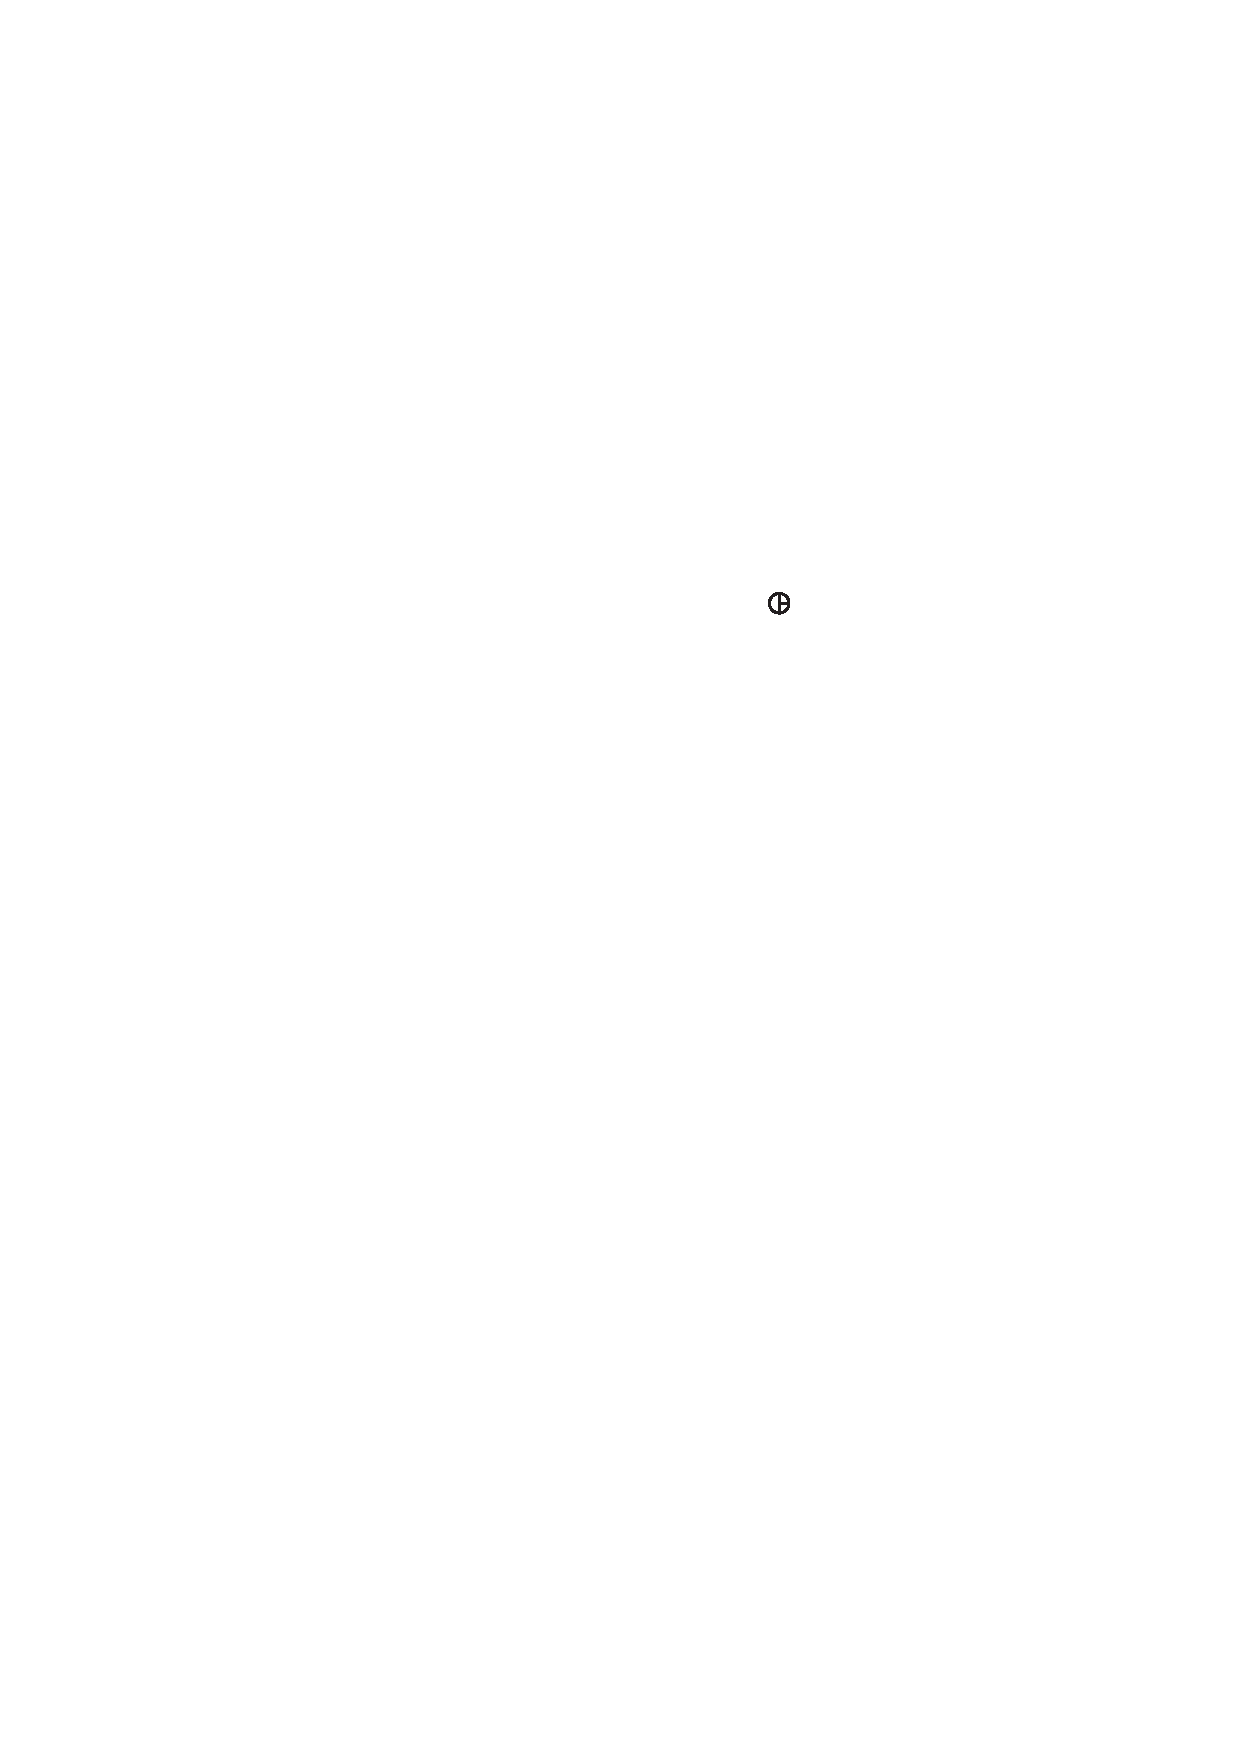
\includegraphics[width=0.02\textwidth]{images/vitriol.pdf}li conjunctionem cum quarta parte Mercurii currentis et hujus in eadem quantitate \pgrk{f}legmatis separationem, vide
\protect\index{Namensregister}{\textso{Van Helmont}, Johan Baptista 1580-1644}\edtext{Helm.}{\lemma{Helm.}\Cfootnote{\textsc{J.B. van Helmont}, \textit{Opuscula medica inaudita}\cite{00522}, K\"{o}ln 1644, S.~72.}}
de Lithiasi c. 4. n. 13.%
%% Hier folgt Bl. 68r.